
\documentclass[11pt]{amsbook}
\usepackage[turkish]{babel}

\usepackage{../Ceyhun}
\usepackage{../amsTurkish}


\usepackage{lipsum}

\begin{document}
	\hPage{059}
	
	\hDefined{Teorem 2.2.1} de ileri sürülen koşul, gerek olmakla birlikte yeterli değildir. Koşulun yetersizliğini bir örnekle aşağıdaki gibi açıklayabiliriz.
	\begin{figure}[htbp]
		\centering
		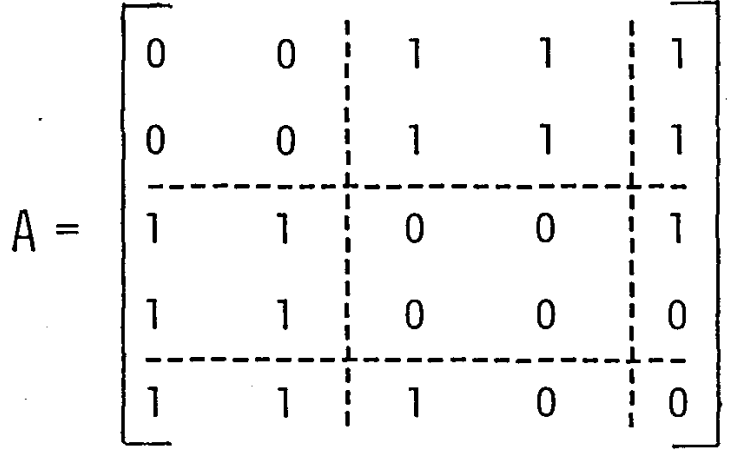
\includegraphics[width=0.45\textwidth]{images/ceyhun-059-fig01.png}
	\end{figure} \\ 
	biçiminde verilen matris,\hDefined{Teorem 2.2.1}deki gerek koşulu sağlamasına karşın, bir çizge ile gerçekleştirilemez. \\
	
	$ Ç(d,a) $ ya ilişkin $a x a$ boyutundaki $A$ matrisi ile $d x a$ boyutundaki $\overline{P}$ matrisini düşünelim. $ A_j, A $ matrisinin ilk $j$ sayıdaki dizek ve dikeçlerinden oluşan altmatrisi, $ \overline{P_j}$ ise $A_j$ altmatrisine ilişkin çakışım matrisini göstersin. Bu durumda, $A_j$ matrisini
	\begin{figure}[htbp]
		\centering
		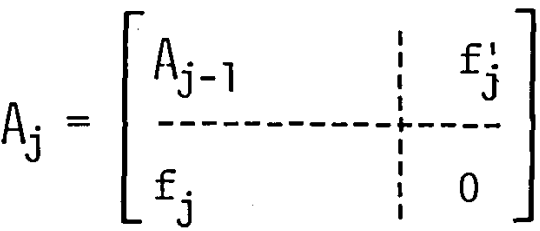
\includegraphics[width=0.45\textwidth]{images/ceyhun-059-fig02.png}
	\end{figure} \\
	olarak yazabiliriz. Burada $f_j,A $ matrsinin $j$ ninci dizeğinde, köşegenine kadar olan ilk $j-1$ teriminin oluşturduğu bir dizek matrisiir. $A_{j-1}$
 

\end{document}